\documentclass{article}
\usepackage[utf8]{inputenc}
\usepackage{mathrsfs}
\title{Numerical Optimization}
\author{jonashj }
\date{January 2021}
\usepackage{optidef}
\usepackage{listings}
\usepackage{natbib}
\usepackage{graphicx}
\usepackage{amsmath}
\usepackage{amssymb}
\usepackage{mathrsfs}
\usepackage{float}
\newcommand{\bm}[1]{\boldsymbol{#1}}
\usepackage{todonotes}

\usepackage[backend = biber,    % Recommended backend for sorting bibliography
            style = authoryear-comp,    % Close to the 'Harvard' referencing style
            urldate = long,     % Long: 24th Mar. 1997 | Short: 24/03/1997
            maxcitenames = 2,   % Number of authors in cite before replaced with 'Author#1 et al.'
            ]{biblatex}
\usepackage[ruled,vlined]{algorithm2e}
\addbibresource{references.bib}     % Adding our file containing the references

\DeclareMathOperator*{\argmax}{arg\,max}
\DeclareMathOperator*{\argmin}{arg\,min}
\begin{document}


\maketitle
\section{Epidemiological Model}
\subsection{SIR}
Due to simple dynamics, the population subject to disease spread is divided into three groups: Susceptible (S), Infected (I) and Recovered(R), yielding the Kermack-Mckendrick model (SIR):
\begin{align}
    \dot{S} &= -\beta \frac{ S I}{N_{pop}}\nonumber\\
    \dot{I} &= \beta \frac{S I}{N_{pop}} - \alpha I\\
    \dot{R} &= \alpha I\nonumber
\end{align}
Where $\beta$ is the infection rate in the population, $\alpha$ is the recovery rate and $N_{pop} = S + I + R$ is the total population.

With respect to optimal control of epidemics, both $\beta$ and $\alpha$ can be controllable depending on the situation. $\alpha$ is determined by the expected recovery time of the population, which  may vary depending on the treatment given to the infected. Modeling of the COVID-19 pandemic is usually done by dividing these three groups into multiple subgroups, yielding more complex models which can be fitted to data. However, the work in this project will only be considering the SIR-model with fixed recovery rate $\alpha$.

The main dynamic of interest is the nonlinear dynamic between the susceptible and infected group, which can be controlled by adjusting $\beta$, or in terms of the expected number of infections per individual, $\mathscr{R}_0$:
\begin{equation}
    \mathscr{R}_0 = \frac{\beta N}{\alpha}
\end{equation}

\subsection{Equilibrium Points}
The number of equilibrium points of the system depends on the reproduction number. When $\mathscr{R}_0 < 1$ the disease does not spread fast enough to beat the recovery rate, and will eventually die out. 
\begin{equation}
    \mathscr{E}_0 = (S_\infty, 0, R_\infty)
\end{equation}
This is the disease-free equilibrium, which is the optimal goal for cumulative infection-minimizing control strategies. In the case of a higher reproduction number, another equlilibrium point occurs through bifurcation (Figure \ref{fig:Forward_Bifurcation}). 
\begin{figure}[h]
    \centering
    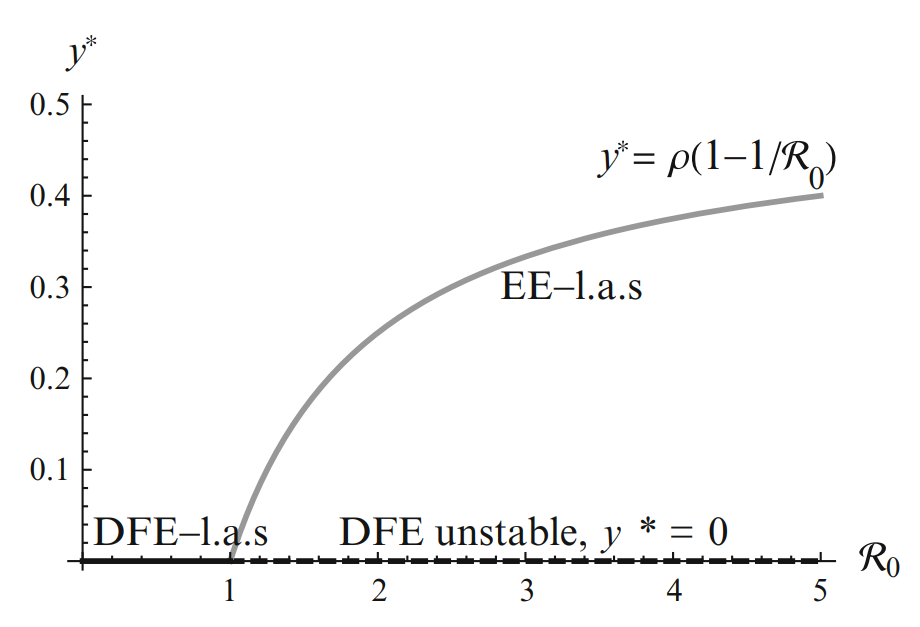
\includegraphics[width = .6\textwidth]{Figures/Bifurkasjonsdiagram_SIR.PNG}
    \caption{Bifurcation-diagram for a dimensionless SIR-model. 
    ($y^*$ is the dimensionless number of infected) [\cite{Martcheva}]}
    \label{fig:Forward_Bifurcation}
\end{figure}

With $\mathscr{R}_0 > 1$ the disease-free equilibrium is unstable. An outbreak will cause temporarily unstable dynamics which will stabilize as the number of susceptibles decrease. The system will converge towards the endemic equilibrium. This equilibrium maximizes the cumulative number of infections.
\subsection{Stability}
\label{ch:SIR_stability}
The local stability in each state can be analyzed with the jacobian of the differential equations:

\begin{equation}
    J = 
    \begin{bmatrix}
    -\frac{\beta I}{N} & \frac{\beta S}{N} & 0\\
    \frac{\beta I}{N} & \frac{\beta S}{N} - \alpha & 0 \\
    0 & \alpha & 0
    \end{bmatrix}
\end{equation}
The three eigenvalues of the jacobian are $\lambda_0 = 0$ and two complex values given by:
\begin{align}
    \lambda_{1,2} &= \frac{\beta(S-I)-\alpha N}{2N}  \pm K\\
\end{align}
The unstable dynamics is given by the real part of the complex eigenvalues, and can be represented by the reproduction number:
\begin{align}
    Re[\lambda_{1,2}] &> 0\\
    \frac{\mathscr{R}_0(S-I)}{N} &> 1
\end{align}
The most unstable eigenvalue occurs when $\mathscr{R}_0 = \mathscr{R}_{0, max}$ and $\max_{S, I} (S-I)$. Since $S$ is monotonically decreasing, this will occur at $(S, I, R) = (S_0, I_0, R_0)$.

\subsection{Control strategies}
Reduction of the number of infected can be achieved using different strategies, including vaccination, quarantine and social distancing measurements. The different types of mitigation will affect the groups in the SIR model differently.  

\subsection{Social Distancing}
In addition to minimization of the total number of infections, a penalty to the strictness of the social distancing policies can be introduced, resulting in the following minimization problem:
\begin{equation}
    \min_{w} \Phi(w) = \min_{u = [u_0, \dots, u_k]} \int_{t=0}^{T_{end}} I^2(t) - W_u u^2(t)
\end{equation}

Where $u$ is given as the reproduction number $\mathscr{R}_0$ in this case. The constant relationship between $N_{pop}, \alpha$ and $\beta$ makes $\mathscr{R}_0$ and $\beta$ only differ in scaling. 

\subsection{Vaccination}
Vaccination can be implemented as a flow rate from the susceptible to the recovered group. 
\begin{align}
    \dot{S} &= -\beta \frac{SI}{N_{pop}} - (\alpha_v S\mbox{ or }  \alpha_v)\\
    \dot{R} &= \alpha I + \alpha_v S
\end{align}
Increased vaccination will be represented as a positive contribution to the objective function. 
\begin{align}
    \begin{split}
    \min_{w} \Phi(w) &= \min_{u = [u_0, \dots, u_k]} \int_{t=0}^{T_{end}} I^2(t) + W_u u^2(t)\\
    u &= \alpha_v
    \end{split}
\end{align}


\subsection{Isolation}
Putting infected individuals in quarantine eliminates their potential infectiousness, and can be viewed as transfering them over to the recovered group.
\begin{align}
    \dot{I} &= \beta \frac{SI}{N_{pop}} - (\alpha + \alpha_q) I\\
    \dot{R} &= (\alpha + \alpha_q) I
\end{align}

Increased quarantine measures will be represented as a positive contribution to the objective function.
\begin{align}
    \begin{split}
    \min_{w} \Phi(w) &= \min_{u = [u_0, \dots, u_k]} \int_{t=0}^{T_{end}} I^2(t) + W_u u^2(t)\\
    u &= \alpha_q
    \end{split}
\end{align}
Quarantine rate range is more difficult to estimate due to underreporting, self-isolation and asymptomatic individuals. 

\subsection{Problem Parameters}
\label{ch:Problem_Parameters}
For social distancing the reproduction number will be lower-bounded by the lowest estimated value from FHI's national report on the spread of covid-19 in Norway (03/02-21,[\cite{FHI_report}]).$\mathscr{R}_0$ will be upper bounded approximately to one of the highest estimates for countries worldwide ([\cite{France_high_R0}]). $\alpha$ will be fixed according to the expected time spent in the infectious class[\cite{Infectious_Period}]. 
\begin{align}
\alpha &= \frac{1}{9[\text{days}]} \approx 0.11\\
\mathscr{R}_0 &\in [0.5, 6.5]
\end{align}

The default time horizon for the control problems is set to $t \in [0, 28] [\text{days}]$. The population size is set approximately to Norways total population ($N_{pop} = 5.3\times 10^6$), and the initial number of infected is set to $2000$. 

As of 24/02-21, a rough average of the vaccination rate is $\approx 2400$ individuals per day over the past five weeks in Norway. The vaccination rate may be modeled as proportional to $S$, or a flat parameter rate. 
\begin{equation}
    \alpha_v \in [0, 3\times2400]
\end{equation}

An arbitrary range of $\alpha_v \in [0, 1], \alpha_q \in [0, 1]$ is set to view the effect of the proportional terms.

Unless stated otherwise, the economical weighting factor $W_u$ is set to a value where the cost-reduction of $u(t)$ is large enough to make an impact on the control strategy. For social distancing it can be chosen according to equation \ref{eq:Wu_sc}.

\begin{equation}
    W_u = \frac{N_{pop}^2}{k(u_{max}-u_{min})^2}
    \label{eq:Wu_sc}
\end{equation}

\subsection{Uncontrolled System}
Figure \ref{fig:SIR_Uncontrolled} shows the epidemic trajectory with maximum reproduction number.

\begin{figure}[H]
    \centering
    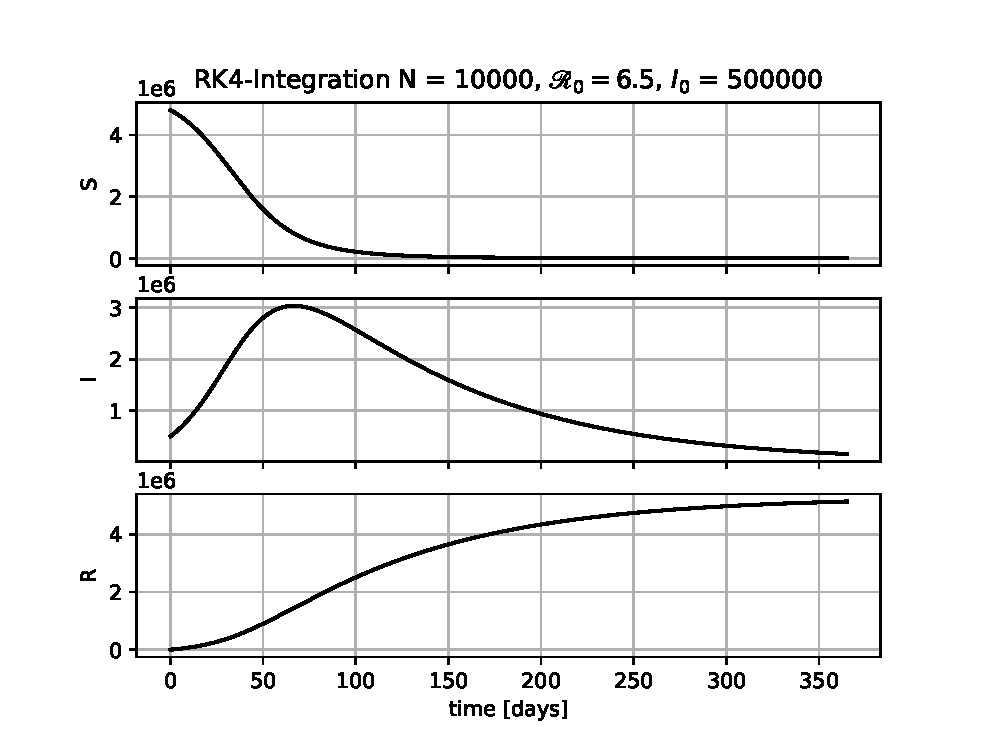
\includegraphics[width=.8\textwidth]{pythonProject/Figures/Uncontrolled_SIR.eps}
    \caption{Uncontrolled SIR-model}
    \label{fig:SIR_Uncontrolled}
\end{figure}

Using a long control horizon the optimal solution(s) have to consider the cost of imposed restrictions against the cumulative number of infected. One challenge with the SIR-model is that the system is asymptotically stable towards the endemic equilibrium in which all individuals have been infected (or vaccinated). The control horizon is too long for any practical purposes, but captures the challenging dynamics of the system. 




\section{Integrators: Explicit Runge-Kutta 4}
A common explicit RK4-scheme is given as:
\begin{align}
    \dot{x} &= F(x,u)\\
    x_{k+1} &= x_k +\frac{h}{6}k_1 + 2k_2 + 2k_3 + k_4\\
\end{align}
With $k$'s given by:
\begin{align}
    k_1 &= F(x_k, u_k)\\
    k_2 &= F(x_k + \frac{h}{2}k_1, u_k)\\
    k_3 &= F(x_k + \frac{h}{2}k_2, u_k)\\
    k_4 &= F(x_k + hk_3, u_k)\\
\end{align}


Yielding the following buther-tableau:
\begin{table}[h]
    \centering
    \begin{tabular}{c|cccc}
         0 & & &  \\
         $\frac{1}{2}$& $\frac{1}{2}$ & &\\ $\frac{1}{2}$& 0 & $\frac{1}{2}$ & &\\
         1 & 0 & 0 & 1 &\\
         \hline &
         $\frac{1}{3}$ & $\frac{1}{6}$ & $\frac{1}{6}$ & $\frac{1}{3}$ 
         
    \end{tabular}
    \caption{RK4 butcher tableau}
    \label{tab:my_label}
\end{table}

Figure \ref{fig:RK4_Stability} shows the stability region of explicit runge-kutta methods.

\begin{figure}[h]
    \centering
    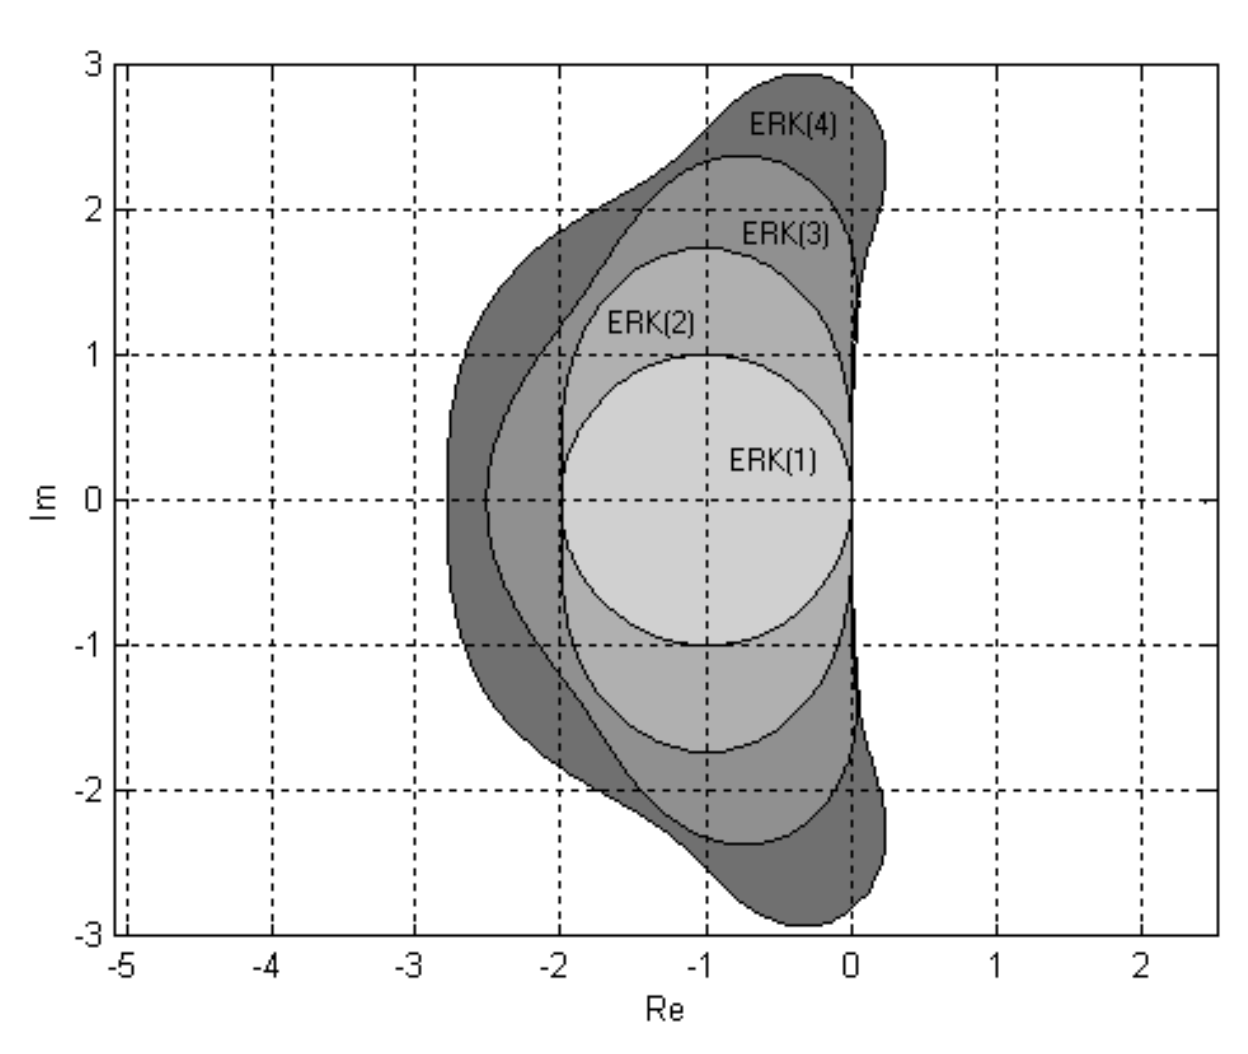
\includegraphics[width=0.8\textwidth]{Figures/RK_Stability_Region.PNG}
    \caption{Runge-Kutta stability regions[\cite{ModSimAuto}]}
    \label{fig:RK4_Stability}
\end{figure}

\subsection{Sensitivities}


\subsubsection{Variational Approach}
General state and input sensitivities can be calculated from partial derivatives of the ODE:
\begin{align}
    \dot{A}(t) &= \frac{\partial F}{\partial x}|_{x(t),u_k} A(t), & &A(t_k) = I\label{eq:sens_A}\\
    \dot{B}(t) &= \frac{\partial F}{\partial x}|_{x(t), u_k} B(t) + \frac{\partial F}{\partial u}|_{x(t), u_k}, & &B(t_k) = 0 \label{eq:sens_B}
\end{align}
Where the ODE for state sensitivity $A(t)$ contains one term, while ODE for input sensitivity $B(t)$ contains two terms due to $u_k$'s indirect impact on $F(t, x, u)$ through $x$. Implementing sensitivities using the variational approach will yield additional integration errors in the extra ODEs (compared to algorithmic differentiation).

\subsubsection{Algorithmic Differentiation}
In algorithmic differentiation, the problem is first discretized, then the sensitivities are obtained from the resulting algorithm. This effectively limits the integration error of the sensitivities to some magnitude of the state integration error.
\begin{algorithm}[H]
\SetAlgoLined
\KwData{$x_k, u_k, h, N$}
 \For{$i$ = 0 : $N-1$}{
    $k_1 = F(x_k, u_k)$\\
    $k_2 = F(x_k + \frac{h}{2}k_1, u_k)$\\
    $k_3 = F(x_k + \frac{h}{2}k_2, u_k)$\\
    $k_4 = F(x_k + hk_3, u_k)$\\
   $x_{k+1} = x_k + \frac{h}{6}k_1 + 2k_2 + 2k_3 + k_4$\\
 }
 \caption{RK4 Integration Algorithm}
\end{algorithm}
The sensitivity equations can be derived using equations \ref{eq:sens_A} and \ref{eq:sens_B}. With full state trajectories provided, the sensitivities can be calculated afterwards according to algorithm \ref{alg:RK4_sense}.

\begin{algorithm}[H]
\SetAlgoLined
\KwData{$[x_0, \dots, x_N], [u_0, \dots, u_N], h, N$}
 \For{$i$ = 0 : $N-1$}{
    $C_x = \frac{\partial}{\partial x}(\frac{h}{6}k_1 + 2k_2 + 2k_3 + k_4)|_{x_k, u_k})$\\
    $C_u = \frac{\partial}{\partial u}(\frac{h}{6}k_1 + 2k_2 + 2k_3 + k_4)|_{x_k, u_k})$\\
    $A_{k+1} = (I + C_x) A_k$\\
    $B_{k+1} = (I + C_x) B_k + C_u B_k$}
 \caption{RK4 Sensitivity Calculation}
 \label{alg:RK4_sense}
\end{algorithm}

Here, the evaluation points are updated with the integrated state, which results in different sensitivity errors than the variational approach. For the upcoming SIR-model, the algorithm will be implemented to yield sensitivities iteratively with the integration.

\subsubsection{Implementation on the SIR-model}
Both approaches require partial derivatives of the SIR-ODE:
\begin{align}
    \frac{\partial F}{\partial x} &= \frac{\partial 
    \begin{bmatrix}
    \frac{-u x_1 x_2}{N_{pop}}\\
    \frac{u x_1x_2}{N_{pop}} - \alpha x_2\\
    \alpha x_2
    \end{bmatrix}
    }{\partial x} = \begin{bmatrix}
    -\frac{ux_2}{N_{pop}} & -\frac{ux_1}{N_{pop}} & 0\\
    \frac{ux_2}{N_{pop}} & \frac{ux_1}{N_{pop}} - \alpha & 0\\
    0 & \alpha & 0
    \end{bmatrix}
    \label{eq:dFdx_SIR}\\
    \frac{\partial F}{\partial u} &= \frac{\partial 
    \begin{bmatrix}
    \frac{-u x_1 x_2}{N_{pop}}\\
    \frac{u x_1 x_2}{N_{pop}} - \alpha x_2\\
    \alpha x_2
    \end{bmatrix}
    }{\partial u} = 
    \begin{bmatrix}
    \frac{-x_1 x_2}{N_{pop}}\\
    \frac{x_1 x_2}{N_{pop}}\\
    0
    \end{bmatrix}
    \label{eq:dFdu_SIR}
\end{align}

Using equations \ref{eq:dFdx_SIR} and \ref{eq:dFdx_SIR}, the two approaches for sensitivity were implemented with the RK4 scheme in Python. Simulating the system with a reproduction number $\mathscr{R}_0 = 10$ and $\alpha = \frac{1}{3}$ (average recovery time of 3 days) yields different results depending on the step time $\Delta t$.

\begin{figure}[h]
    \centering
    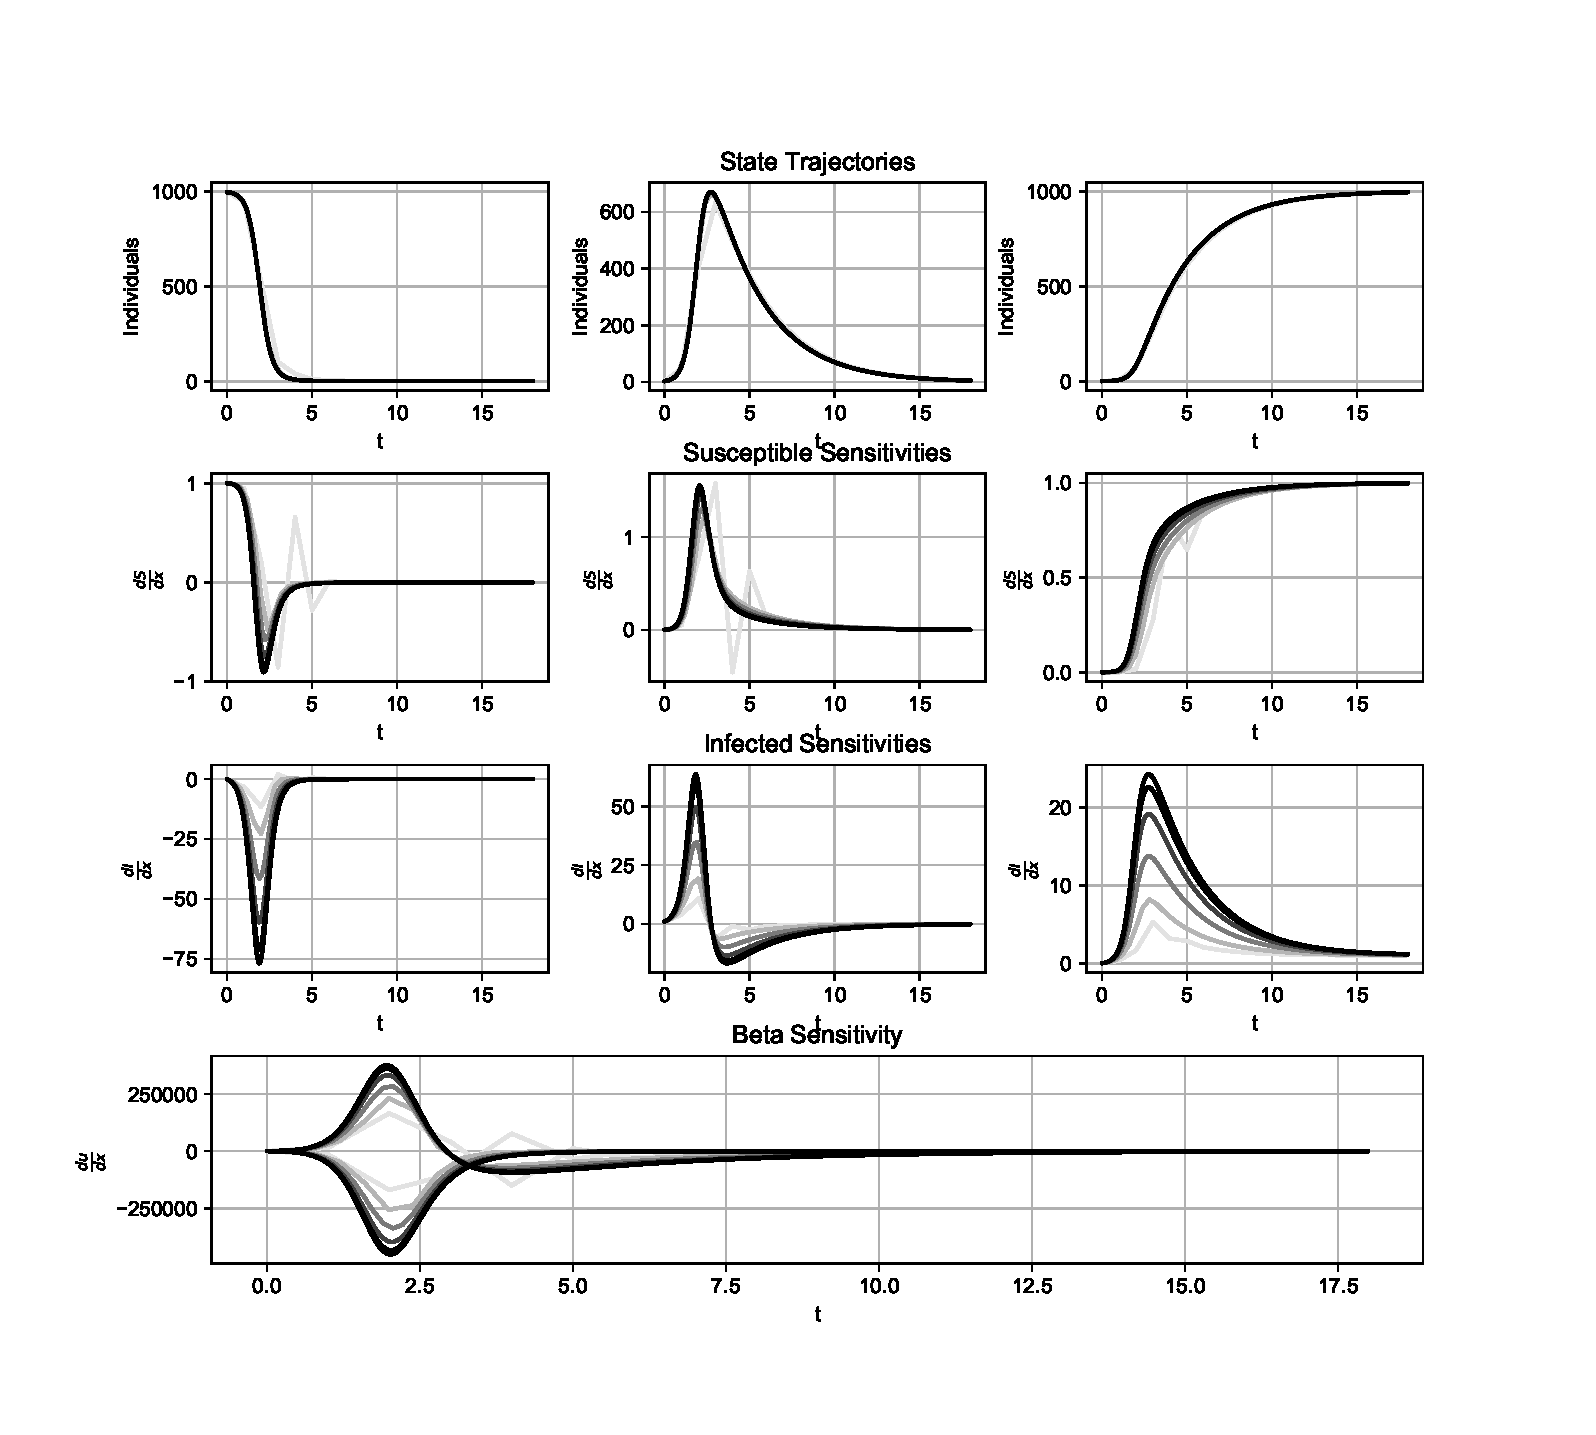
\includegraphics[width=.9\linewidth]{Figures/Autodiff_Sensitivities.eps}
    \caption{RK4-scheme sensitivities and trajectories with autodifferentiation. $\Delta t = [1.        , 0.39810717, 0.15848932, 0.06309573, 0.02511886,
       0.01      ]$ gradually colored from white to black}
    \label{fig:RK4_Autodiff}
\end{figure}

The susceptible and infected sensitivities with respect to the susceptible and infected populations (plots $[1:2,1:2]$) show that the most fragile timepoints of the epidemic occurs when the product of susceptibles and infected are highest. The third column shows sensitivities with respect to the recovered individuals.

Even though automatic differentiation should present a smaller integration error, it was not possible to find visible differences between the two approaches using stepsizes down to $\Delta t = 1e-5$. When compared to the 'true' trajectories, they presented the same errors.

\subsection{Bounds and Nonlinearity}
The SIR-model itself is a Lipschitz, continously differentiable ODE which with the variational RK4-scheme approach also has continous dynamics for the sensitivities. It is visible in figure \ref{fig:RK4_Autodiff} that the maximum sensitivities of the susceptible and infected states are found at $S = I$ for $\mathscr{R}_0 > 1$. Values at this point is found at the equilibrium point of the sensitivity equations:

\begin{align}
        &\frac{\partial F}{\partial x}|_{x(t),u_k} A(t) = 0\\
 &\frac{\partial F}{\partial x}|_{x(t), u_k} B(t) + \frac{\partial F}{\partial u}|_{x(t), u_k} = 0
\end{align}

State $R$ can be excluded from the analysis, yielding a $2\times 2$ analysis:

\begin{equation}
\frac{\partial F}{\partial x}|_{x(t),u_k} A(t) = 
\begin{bmatrix}
    a_{12}\,u\,x_{2}-a_{11}\,u\,x_{1} & -a_{12}\,\left(\alpha-u\,x_{1}\right)-a_{11}\,u\,x_{1}\\ a_{22}\,u\,x_{2}-a_{21}\,u\,x_{2} & -a_{22}\,\left(\alpha-u\,x_{1}\right)-a_{21}\,u\,x_{1} 
    \end{bmatrix}
\end{equation}
Inserting the 


\subsubsection{Instability and Step Length}
As shown in \ref{ch:SIR_stability} the SIR-model will have local unstable dynamics, which in turn cause unstable integration errors. The errors will have to be restricted using small enough integration steps. The instability of the integrator can be determined by:
\begin{equation}
    R_{E, max}(\lambda \Delta t) = det[I-\text{Re}_{max}[\lambda_{1,2}] \Delta t(A - 1b^T)]
\end{equation}
Where $A$ and $b$ is given by the buther tableau. Inserting the eigenvalue corresponding to the most unstable dynamic achieveable, this yields:
\begin{equation}
    R_{E, max}(\lambda \Delta t) = det[I- \frac{\beta_{max}(S_0-I_0) - \alpha}{2N} \Delta t(A - 1b^T)]
\end{equation}
\subsection{Integrators: Collocation}
A collocation integrator constructs the trajectory using
parameters $\theta$ on a time grid of $d+1$ points in $[t_k, t_{k+1})$ ($[\tau_0, \tau_1, \dots, \tau_d]$). Parameters $theta$ are constrained to equal the value of the trajectory at these points, giving the full trajectory as a sum of lagrange polynomials:
\begin{align}
    P_i(\tau) &= \prod_{j=0, j \neq i}^{d+1} \frac{\tau-\tau_j}{\tau_i - \tau_j}\\
    s_k(\theta, \tau) &= \sum_{j=0}^{d+1} \theta_j P_j(\tau)
\end{align}
Matrices $C \in \mathbb{R}^{(d+1)\times(d+1)}$ and $B, D \in \mathbb{R}^{(d+1)}$ can be constructed, respectively containing coefficients for the derivatives and the end state for the polynomials. This makes it possible to calculate $\bm{\theta}$, $\bm{\dot{\theta}}$ and the objective value accumulated over each timestep $t_k$. Figure \ref{fig:Lagrange_Polynomials} illustrates the properties of the coefficients.

\begin{figure}[h]
    \centering
    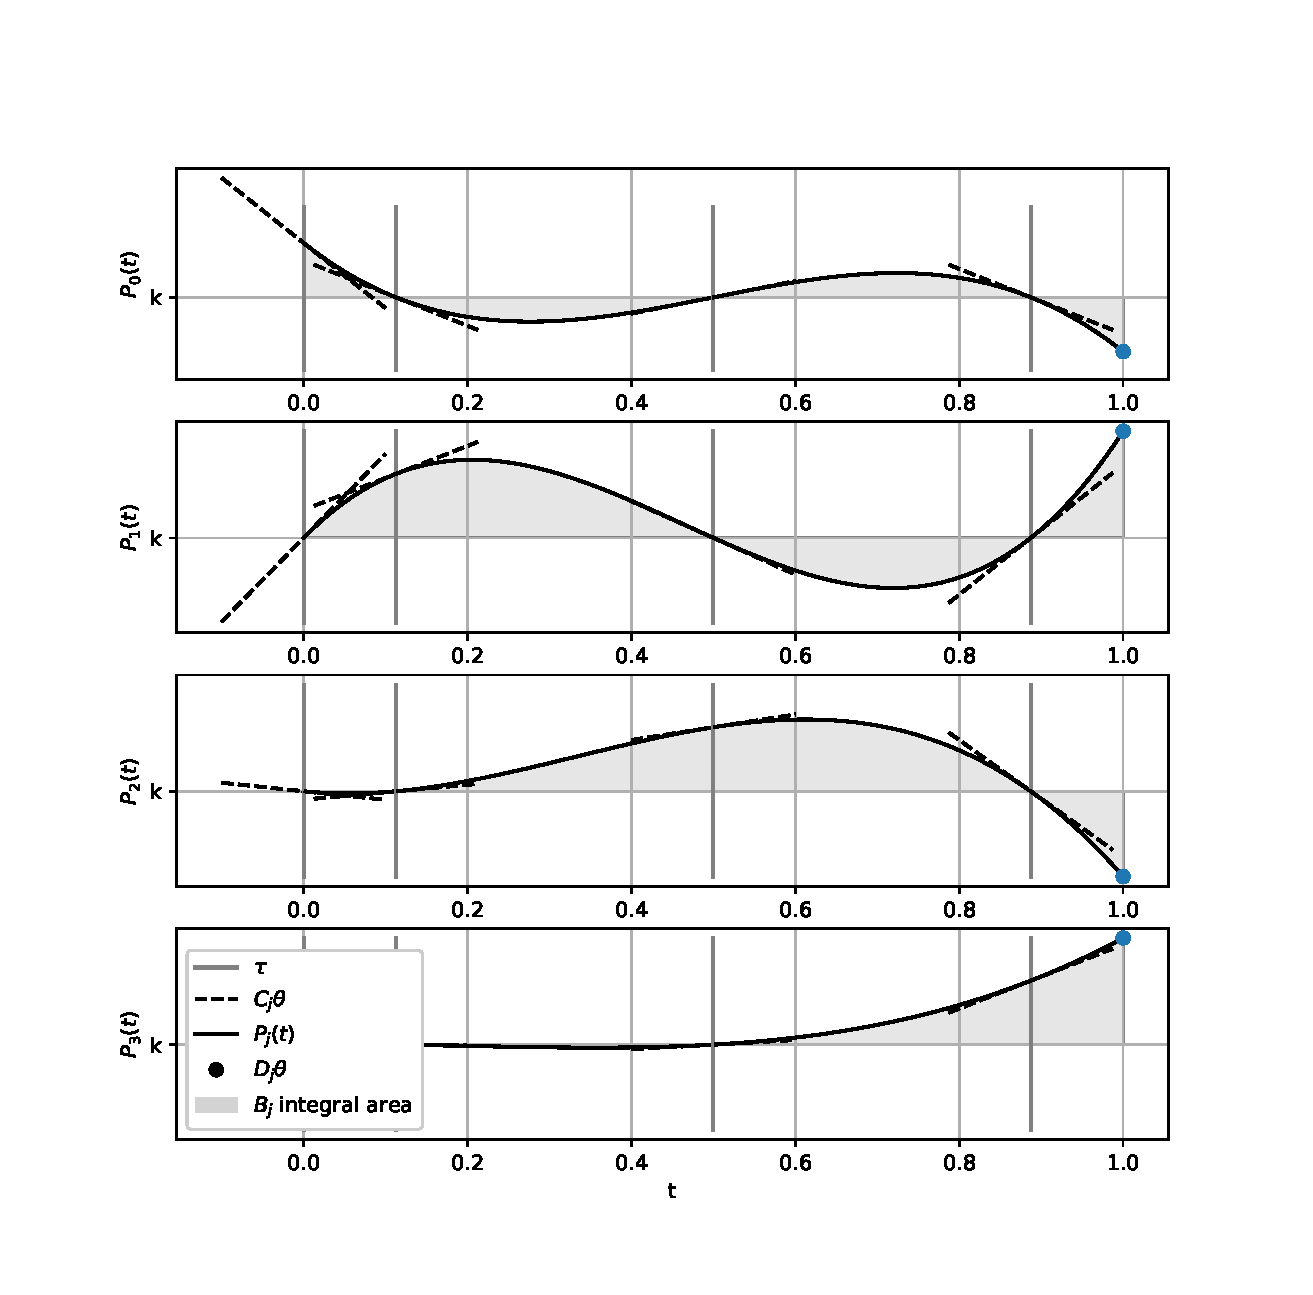
\includegraphics[width=1\textwidth]{Figures/lagrange_polynomial.eps}
    \caption{Lagrange Polynomials using legendre-timepoints for $d=3$}
    \label{fig:Lagrange_Polynomials}
\end{figure}

The derivative of the trajectory can be constrained to match the ODE in order to approximate the true trajectory at the chosen timepoints:
\begin{align}
    g_{\text{col}} &= \dot{s}_k(\theta, \tau) - F(\theta_i, t_k + \tau_i) = \sum_{j=0}^{d+1}\theta_j\dot{P}_j(t_k + \tau_i)  - F(\theta_i, t_k + \tau_i) = 0\\ \forall k, i &\in [0,\dots, N-1], [0, \dots d]\nonumber
\end{align}
\subsubsection{Sensitivities}
$g_{col} = 0$ can be solved with newton-raphson, yielding $\frac{\partial g_{col}}{\partial \theta}$ as a biproduct. The sensitivities of the integrator with respect to state and control input can be derived from the implicit function theorem, yielding:
\begin{align}
    \frac{\partial \theta}{\partial x} &= \frac{\partial g_{col}}{\partial \theta}^{-1}\frac{\partial g_{col}}{\partial x} &     \frac{\partial \theta}{\partial u} &= \frac{\partial g_{col}}{\partial \theta}^{-1}\frac{\partial g_{col}}{\partial u}
\end{align}




\section{Single Shooting}
The optimization problem can be formulated as an nlp with the system dynamics as constraints. To avoid persistent strict policies, the cost function decreases quadratically with $u_k$. This can be viewed as a penalty modelling the negative impacts of lockdown.

\begin{mini*}|s|
{w}{\sum_{k=1}^NI_k^2 -W_u u_{k-1}^2 \triangleq \Phi(w)}
{}{}
\addConstraint{x_f = f(x_0, [u_0, \dots, u_{N-1}])}
\addConstraint{u_{max} \geq u_k \geq u_{min}}{}
\end{mini*}
Where $f(.)$ is the trajectory from initial to end state. The intermediate states of the system is not visible to the solver. $f(.)$ can be implemented as an iterative RK4-scheme:

\begin{algorithm}[H]
\SetAlgoLined
\KwData{$x_k = x_0, u = [u_0, \dots, u_{N-1}], h, N$}
define f as a RK4-integrator repeated M times\\
 \For{$i$ = 0 : $N-1$}{
    $x_k, Q_k = RK4(@SIR,@Cost, x_k, u_k, h)$\\
    $J += Q_k$\\
    add $u_{min} - u_k, u_k - u_{max}$ to bounds\\
    set $u_{k,0}$
 }
 \KwRet{$x_k, J, U_0$, bounds}
 \caption{Single-shooting problem construction and integration}
 \label{alg:SingleShooting_Integraion}
\end{algorithm}

The resulting variables, values and boundaries can be directly inserted into the CasADI-interface if derived symbolically, or directly intefaced with a solver when derived numerically.
\iffalse
\subsection{Optimal Control using IPOPT interfaced by CasADI}
The problem is formulated using CasADI in Python, where a single step of algorithm \ref{alg:SingleShooting_Integraion} is formulated with MX-symbolics and transformed to a CasADI-function. $u = [u_0, \dots, u_{N-1}]$ is initialized as a MX-variable and elementwise inserted into the function for each for-loop step in algorithm \ref{alg:SingleShooting_Integraion}. Boundaries are added to $u$, resulting in lists which can be inserted into the CasADI's solver framework.

Optimal control is solved using default parameters and initial conditions from \ref{ch:Problem_Parameters}.

\fi



\subsection{Primal-Dual Interior Point Formulation}
\subsubsection{KKT Conditions}
The inequalities can be replaced using the log-barrier method:

\begin{mini*}|s|
{w_\tau}{\Phi(w_\tau) - \tau \sum_{k=0}^{N-1}(\log(u_k-u_{min}) + \log(u_{max}-u_k))}
{}{}
\addConstraint{x_f = f(x_0, [u_0, \dots, u_{N-1}])}
\end{mini*}
\begin{align}
    h(w_\tau) &= \begin{bmatrix} u_0-u_{min} \\ u_{max}-u_0 \\ \vdots \\
u_{max}-u_{N-1}
    \end{bmatrix}& 
 \nu&= -\tau \begin{bmatrix}
h_0^{-1}\\ \vdots \\ h_{2(N-1)}^{-1} \end{bmatrix}
\end{align}
Which gives the Primal-Dual KKT-conditions:
\begin{align}
    \nabla \Phi(w) + \nabla h(w)\nu + \nabla f(x_0, [u_0, \dots, u_{N-1}])\lambda &= 0\nonumber \\
    g(w) = x_f-f(x_0, [u_0, \dots, u_{N-1}]) &= 0\\\nonumber
    \nu_ih_i(w) + \tau &= 0 \\\nonumber
    h(w) < 0, \nu &> 0
\end{align}
The complementarity slackness in the Primal-Dual method approximates the constraints for the original formulation, and will converge to $\mu$ for small $\tau$. The current formulation requires $h(w) < 0$, which can be relaxed with slack variable $s$. Furthermore, the problem can be expressed in terms of true KKT conditions by setting $\nu = \mu$, which upper bounds the optimum error $\mu^*-\nu^*$ linearly with $\tau$. This results in equation \ref{eq:KKT_approx_IPOPT}, where the equalities can be used for Newton-Rhapson steps.

\begin{align}
        \nabla \Phi(w) + \nabla h(w)\nu + &\nabla f(x_0, [u_0, \dots, u_{N-1}])\lambda = 0 \nonumber \\ 
        g(w) &= 0\nonumber \label{eq:KKT_approx_IPOPT}\\
    h_i(w) + s_i &= 0\\\nonumber
    \mu_is_i-\tau &= 0\\\nonumber
    s > 0, \mu &> 0
\end{align}

\subsubsection{Line Search}
In the case where the end-state of the trajectory is unconstrained, $g(w)$ can be omitted. The solution for each KKT problem can be found by using the Newton-Rhapson method on the KKT conditions. 
\begin{align}
    r(w, \mu, \tau) &= \begin{bmatrix}
    \nabla \mathcal{L}(w, \mu)\\
    h(w) + s\\
    \mu_is_i - \tau
    \end{bmatrix} = 0\\
    \begin{bmatrix}
    d^w\\d^\lambda\\d^\mu
    \end{bmatrix} &= \nabla r(w, \mu, \tau)^{-1} r(w, \mu, \tau)
\end{align}

It is not possible to guarantee invertibility of $r$ for the SIR-model due to nonlinear dynamics. [\cite{IPOPT_output_ref}] suggests ensuring invertibility by adding a diagonal term $\delta_w$ to the hessian of the lagrangian $\nabla_{ww}\mathcal{L}(w, \mu)$ in $\nabla r(w,\mu, \tau)$.

The steps can be constrained to decrease $r(w, \mu, \tau)$ at every iteration with the fraction-to-the-boundary rule:
\begin{align}
    \alpha_k^{max} &= \max \{\alpha \in (0,1]: w_k + \alpha d_k^w \geq (1-\tau_j)x_k\}\\
     \alpha_k^{\mu} &= \max \{\alpha \in (0,1]: \mu_k + \alpha d_k^\mu \geq (1-\tau_j)\mu_k\}\\
\end{align}
Where $w$ and $\lambda$ are updated according to $\alpha_k^{max}$, and $\mu$ according to $\alpha^\mu$.



\subsection{Sequential Quadratic Programming Formulation}
The problem can be approximated using the hessian of the lagrangian combined with the gradient of the objective, constraint and inequalities:
\begin{align}
    \mathcal{L}(x, \lambda, \mu) = \sum_{k=1}^NI_k^2 -W_u u_{k-1}^2 - \lambda g(w) - \mu h(w)
\end{align}

\begin{mini}|s|
{d}{\frac{1}{2}d^T \nabla^2_{ww}\mathcal{L}\mathcal(w) d + \nabla \Phi(w)^T d}
{}{}
\addConstraint{\nabla g(w)^T d + g(w) = 0}
\addConstraint{\nabla h(w)^T d + h(w) \leq 0}{}
\end{mini}
\subsubsection{Active Set Strategy}
After determining the current active inequality constraints, the the sequential step and multipliers can be determined from the Karush-Kuhn-Tucker conditions of the problem (Considering the approximated active inequalities $\nabla h_A(w)^T d + h_A(w) \leq 0$ as equality constraints with multiplier $\mu$).
\begin{equation}
    \begin{bmatrix}
    \nabla_{ww}\mathcal{L}(w, \lambda, \mu) & \nabla g(w) & \nabla h_A(w)\\
    \nabla g(w)^T & 0 & 0\\
    \nabla h_A(w)^T & 0 & 0
    \end{bmatrix}
    \begin{bmatrix}
    d\\
    \lambda\\
    \mu_A
    \end{bmatrix}= 
    -\begin{bmatrix}
    \Phi(w)\\
    g(w)\\
    h_A(w)
    \end{bmatrix}
\end{equation}

In the SIR-problem formulation we have the following boundary inequalities:
\begin{align}
    h(w) &= \begin{bmatrix} u_0-u_{min} \\ u_{max}-u_0 \\ \vdots \\
u_{max}-u_{N-1}
    \end{bmatrix} & \nabla h(w) &= \begin{bmatrix} 1 \\ -1 \\ \vdots \\1\\
-1
    \end{bmatrix}
\end{align}
Determining the active set for boundaries is simpler than for other inequalities, since they come in pairs where only one can be active at each iteration.

In the case of independent inequality constraints, the active set has to be determined by testing different steps with different active inequalities until positive multipliers and a feasible step has been achieved.

\subsection{IPOPT with CasADI's Symbolical Framework}
A single-shooting optimization problem was formulated with CasADI using the symbolical framework, for all three control strategies. Algorithm \ref{alg:PDIPOPT_CasADI_SYM} summarizes the basic loop for converging without $\delta$ or step-corrections.


\begin{algorithm}[H]
\SetAlgoLined
\KwData{$w = w_0 \in \mathbb{R}^{N_u + N_\mu + N_s}, \tau = 1, \tau_{min} = 1\times 10^{-3}, \Delta w_{tol} = 1\times 10^{-4}$}
\While {$(\tau > \tau_{tol})$ and $(\Delta w > \Delta w_{tol})$}{

    \While {$w_k > w_{k, tol}$}{

        $w_k = w_k - \nabla r(w, \mu, \tau)^{-1} r(w, \mu, \tau)$


    \EndWhile}

    $\Delta w = w_k - w_{k, old}$

    $\tau = 0.9\tau$

\EndWhile}

 \KwRet{$w_k$}
 \caption{Primal-Dual Interior Point with CasADI symbolical framework}
 \label{alg:PDIPOPT_CasADI_SYM}
\end{algorithm}

\subsubsection{Social Distancing}

Reducing step lengths using the fraction-to-the-boundary rule resulted in a very slow convergence with very small steps in $\alpha_k^\mu, \alpha_k^{max}$. While using $\delta$ and small steps is keeping $\nabla r(w, \mu, \tau)$ invertible, it does not converge towards a local optimal solution.

\subsubsection{Vaccination}

Optimization with vaccination policy was solvable without $\delta$ and step-corrections.

\begin{figure}[H]
    \centering
    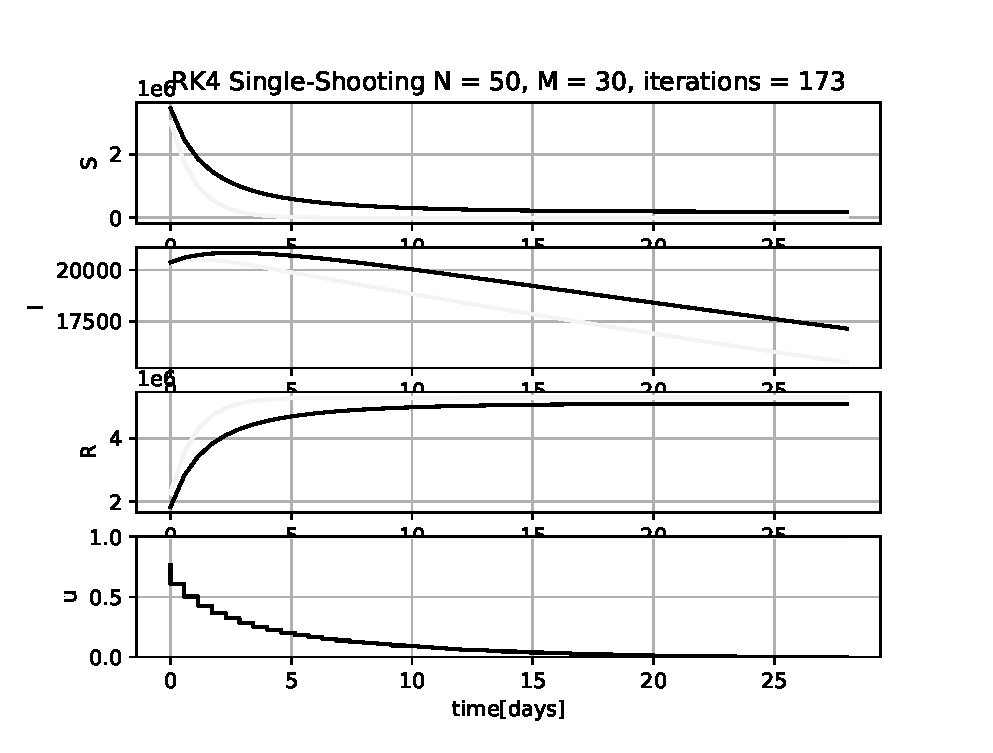
\includegraphics[width=.8\textwidth]{pythonProject/Figures/Symbolic_IPOPT_Traj_Vaccination.eps}
    \caption{Vaccination trajectories using Symbolical DP-IPOPT}
    \label{fig:Symbolical_DPIPOPT_traj_Vaccine}
\end{figure}
Figure \ref{fig:Delta_wk_convergence_Vaccine} shows the convergence of $\Delta w_k$.

\begin{figure}[H]
    \centering
    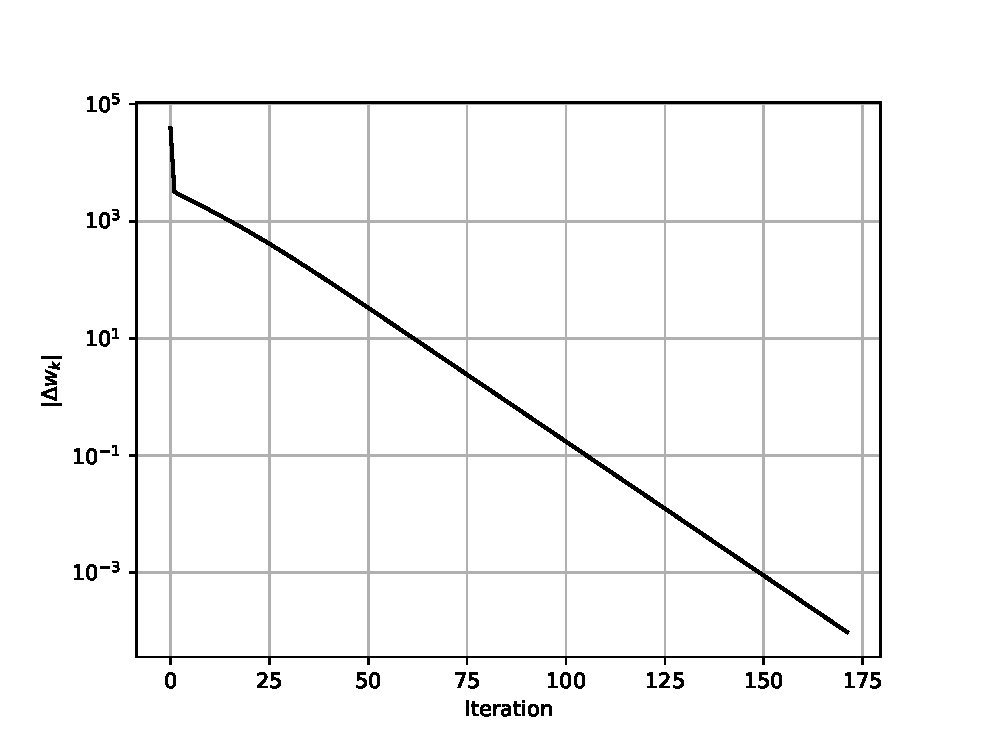
\includegraphics[width=.8\textwidth]{pythonProject/Figures/Symbolic_IPOPT_error_Vaccination.eps}
    \caption{$\Delta w_k$-convergence (Vaccine)}
    \label{fig:Delta_wk_convergence_Vaccine}
\end{figure}

\subsubsection{Isolation}

Optimization with isolation policy was solvable without $\delta$ and step-corrections.

\begin{figure}[H]
    \centering
    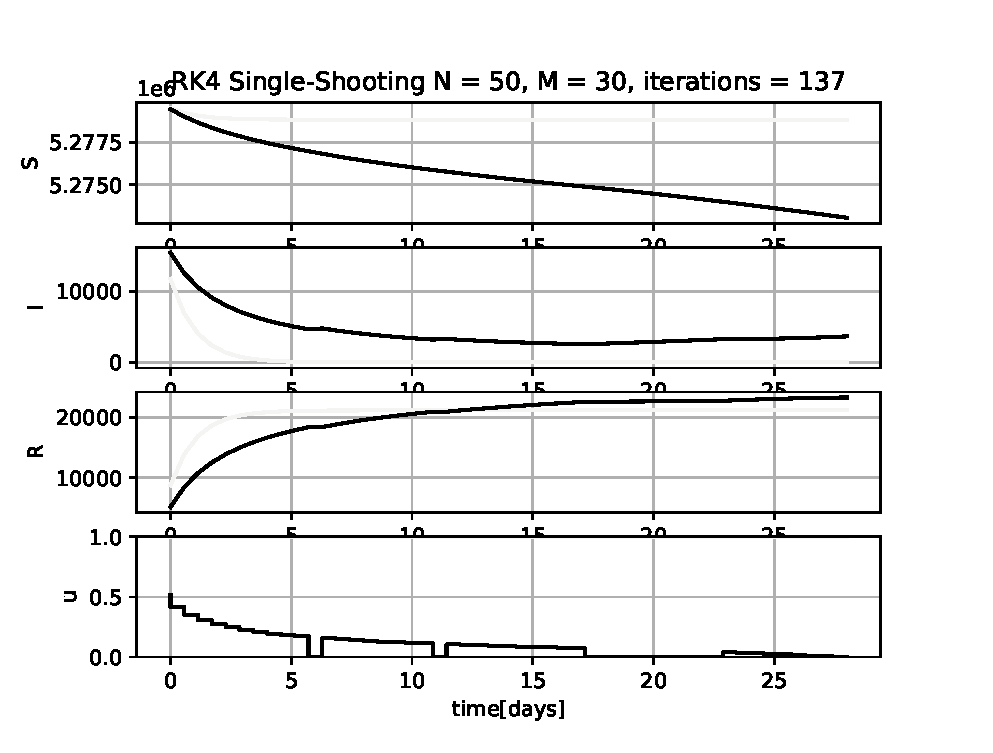
\includegraphics[width=.8\textwidth]{pythonProject/Figures/Symbolic_IPOPT_Traj_Isolation.eps}
    \caption{Isolation trajectories using Symbolical DP-IPOPT}
    \label{fig:Symbolical_DPIPOPT_traj_Vaccine_Isolation}
\end{figure}
Figure \ref{fig:Delta_wk_convergence_Isolation} shows the convergence of $\Delta w_k$.

\begin{figure}[H]
    \centering
    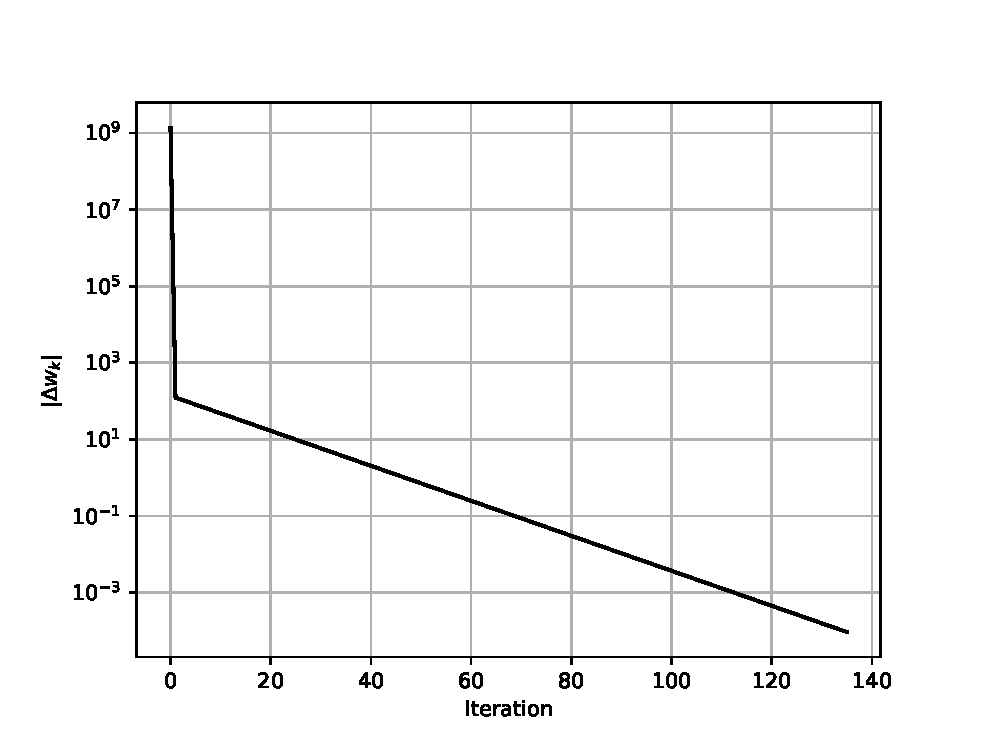
\includegraphics[width=.8\textwidth]{pythonProject/Figures/Symbolic_IPOPT_error_Isolation.eps}
    \caption{$\Delta w_k$-convergence (Isolation)}
    \label{fig:Delta_wk_convergence_Isolation}
\end{figure}


\subsection{Interfacing IPOPT in CasADI}
\subsubsection{Implementation}
Single-shooting is implemented in CasADI using $X_0 \in \mathbb{R}^3, U \in \mathbb{R}^{N}$ as MX-variables. The ODE is integrated $M$ times for each control interval, resulting in a total of $N\times M$ integration steps. Inequality constraints are passed as variable bounds, while equality constraints are passed as regular constraints to the solver.

\begin{algorithm}[H]
\SetAlgoLined
\KwData{$x_k = x_0, U = MX \in \mathbb{R}^{N}, J=0, h, N$}
Construct integrator $f(ODE, x, u, h)$ with CasADI-symbolics\\
 \For{$i$ = 0 : $N-1$}{
    $x_k, Q_k$ = $f([@SIR, @Cost\_ODE], x_k, U[i], h)$\\
    $J+= Q_k$\\
    add $u_{min} - u_k, u_k - u_{max}$ to bounds\\
    set $u_{k,0}$
 }
 solver = nlpsol('solver', 'ipopt', $\{$J, $U\}$)\\
 sol = solver($U_0$,bounds)
 \caption{Single-shooting with IPOPT}
 \label{alg:SingleShooting_Integration_IPOPT}
\end{algorithm}
\subsubsection{Social Distancing}
Simulating with parameters defined in section \ref{ch:Problem_Parameters} yields trajectories shown in figure \ref{fig:SH_Traj_IPOPT} and multiplier and objective values shown in figure \ref{fig:SH_con_obj_IPOPT}.

\begin{figure}[H]
    \centering
    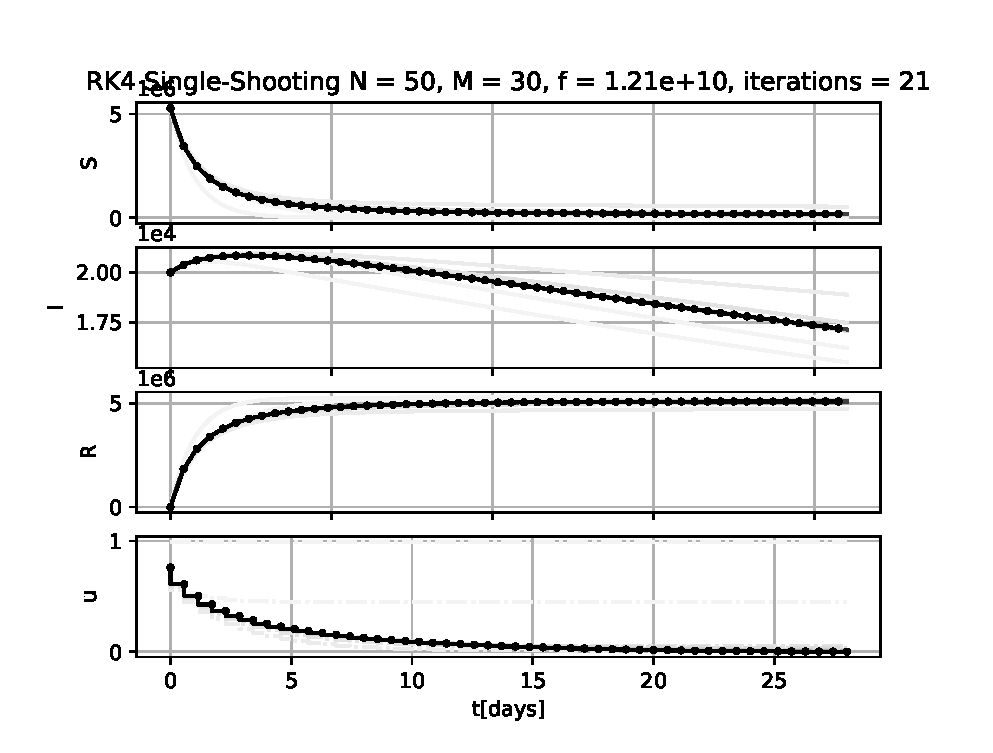
\includegraphics[width=.8\textwidth]{pythonProject/Figures/Single_Shooting_Trajectory_IPOPT.eps}
    \caption{Trajectories with single shooting using IPOPT}
    \label{fig:SH_Traj_IPOPT}
\end{figure}

\begin{figure}[H]
    \centering
    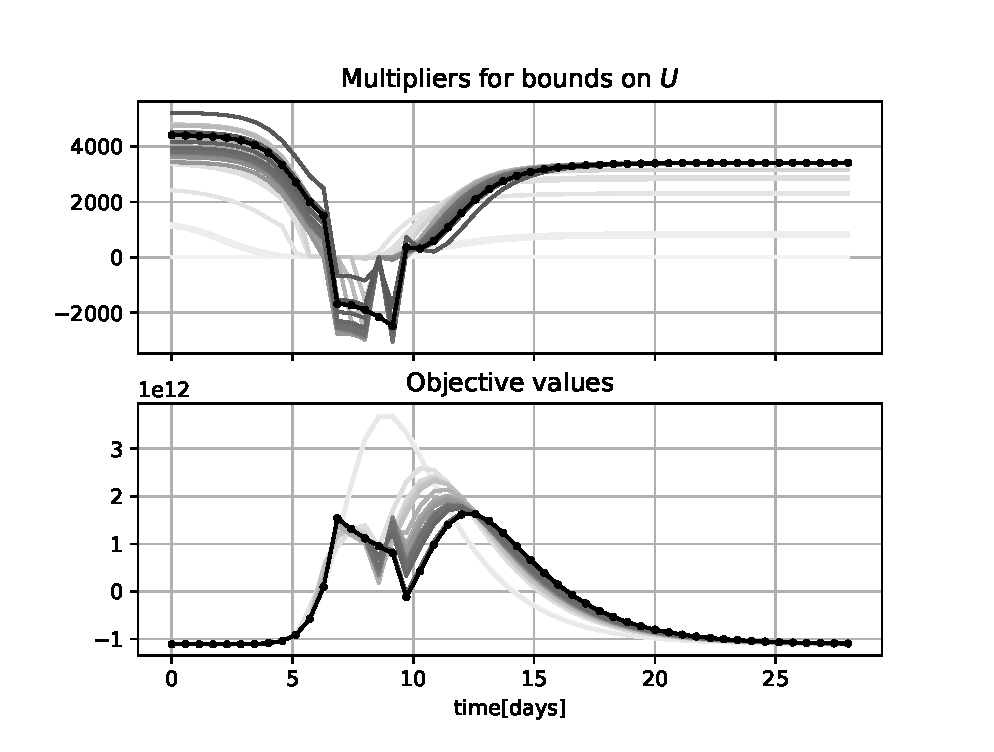
\includegraphics[width=.8\textwidth]{pythonProject/Figures/Single_Shooting_obj_con_IPOPT.eps}
    \caption{Bounds multipliers and objective values for single shooting using IPOPT (Social Distancing)}
    \label{fig:SH_con_obj_IPOPT}
\end{figure}
It is clear that the most cost-critical region $t\in [5, 10]$ is considered by the solver when it is searching for a solution. This region contains the highest objective values for the early iterations. The first iterations drastically reduce the objective values, 

\textbf{Note:} The IPOPT documentation does not explicitly explain the implementation of bounds, but the solver ensures that the optimization variables stays within them for all iterations. There is one multiplier for each pair of bounds, where the activeness of the bound is determined by the sign of the multiplier.

\subsection{Interfacing SQPOASES in CasADI}
\subsubsection{Implementation}
Passing 'sqpmethod' to $nlpsol(.)$ makes it possible to solve the same problem formulation as algorithm \ref{alg:SingleShooting_Integration_IPOPT}.

\subsubsection{Results}
Simulating with parameters defined in section \ref{ch:Problem_Parameters} yields trajectories shown in figure \ref{fig:} and multiplier and objective values shown in figure \ref{fig:SH_con_obj_IPOPT}.
\section{Multiple Shooting}
\begin{mini*}|s|
{w}{\sum_{k=1}^NI_k^2 -W_u u_{k-1}^2}
{}{}
\addConstraint{f(x_0, u_0) - x_1 = 0}
\addConstraint{f(x_k, u_k) - x_{k+1} = 0}
\addConstraint{\vdots}
\addConstraint{f(x_{N-1}, u_{N-1}) - x_{N} = 0}
\addConstraint{u_{max} \geq u_k \geq u_{min}}{}
\end{mini*}
Where $f(.)$ is the trajectory from $x_k$ to $x_{k+1}$. The RK4-integrator can be replaced by collocation constraints resulting in a direct collocation scheme.

\subsection{Interfacing IPOPT in CasADI}

\subsubsection{Implementation}
\begin{algorithm}[H]
\SetAlgoLined
\KwData{$x = MX \in \mathbb{R}^{N+1}, u = \in \mathbb{R}^{N}, h, N, M$}
define f as chosen integrator

add initial condition bounds
 \For{$i$ = 0 : $N-1$}{
    $x_{int}, Q_k = f(@SIR,@Cost, x_k, u_k, h)$\\
    $J += Q_k$\\
    add $u_{min} - u_k, u_k - u_{max}$ to bounds\\
    add $x_{min}-x_k, x_k - x_{max}$ to bounds\\
    add $x_{int} - x_{k+1}$ to constraints\\
    set $u_{k,0}$\\
    set $x_{k, 0}$
 }
 \KwRet{$x_k, J,X_0,U_0$, bounds, constraints}
 \caption{Multiple-Shooting problem construction and integration (RK4)}
 \label{alg:MultipleShooting_Integraion}
\end{algorithm}

In order to get comparable performance to single shooting, the multiple shooting scheme should be initialized with the same initial trajectory for the lifted states.
\subsubsection{Results (RK4)}
Simulating with parameters defined in section \ref{ch:Problem_Parameters} yields trajectories, bounds multipliers, constraints multipliers and objective values respectively shown in figure \ref{fig:MS_Traj_SD_IPOPT}, \ref{fig:MS_Bounds_SD_IPOPT}, \ref{fig:MS_Cons_Obj_IPOPT} (Using the same initial trajectory as in single shooting). In order to illustrate the advantages of lifting the states, another simulation can be run using $x_0$ as initial value for all lifted states.

\begin{figure}[H]
    \centering
    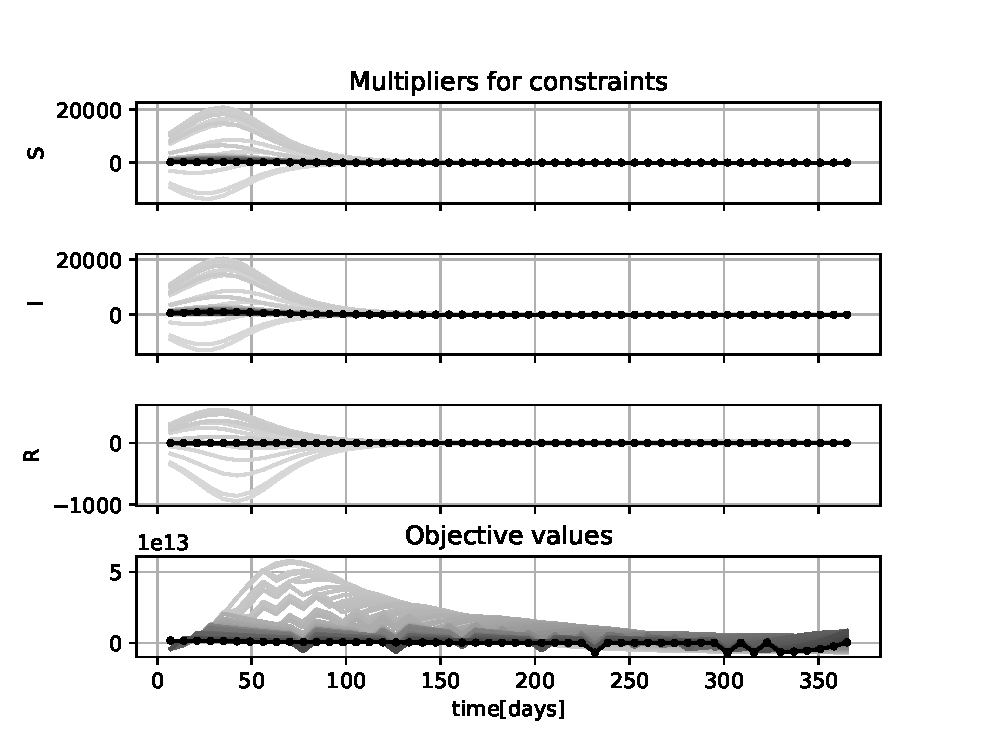
\includegraphics[width=.8\textwidth]{pythonProject/Figures/Multiple_Shooting_obj_con_IPOPT_traj_initial_Social_Distancing.eps}
    \caption{Trajectories with multiple shooting using IPOPT (Social Distancing)}
    \label{fig:MS_Traj_SD_IPOPT}
\end{figure}

\begin{figure}[H]
    \centering
    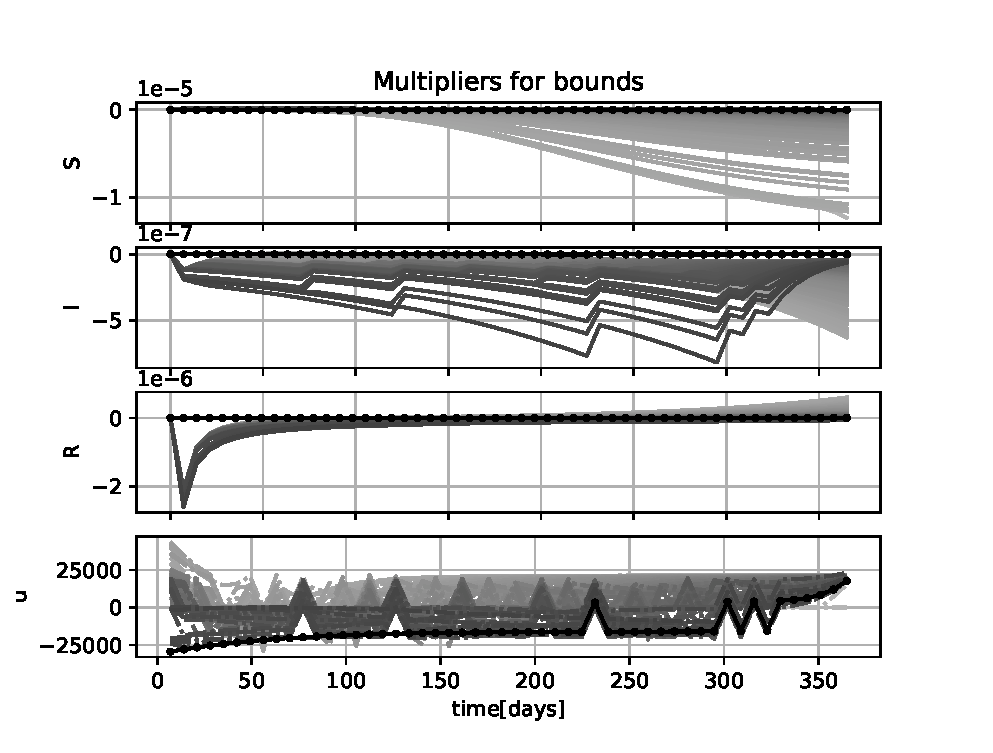
\includegraphics[width=.8\textwidth]{pythonProject/Figures/Multiple_Shooting_bounds_IPOPT_traj_initial_Social_Distancing.eps}
    \caption{Boundary multipliers with multiple shooting using IPOPT (Social Distancing)}
    \label{fig:MS_Bounds_SD_IPOPT}
\end{figure}


\begin{figure}[H]
    \centering
    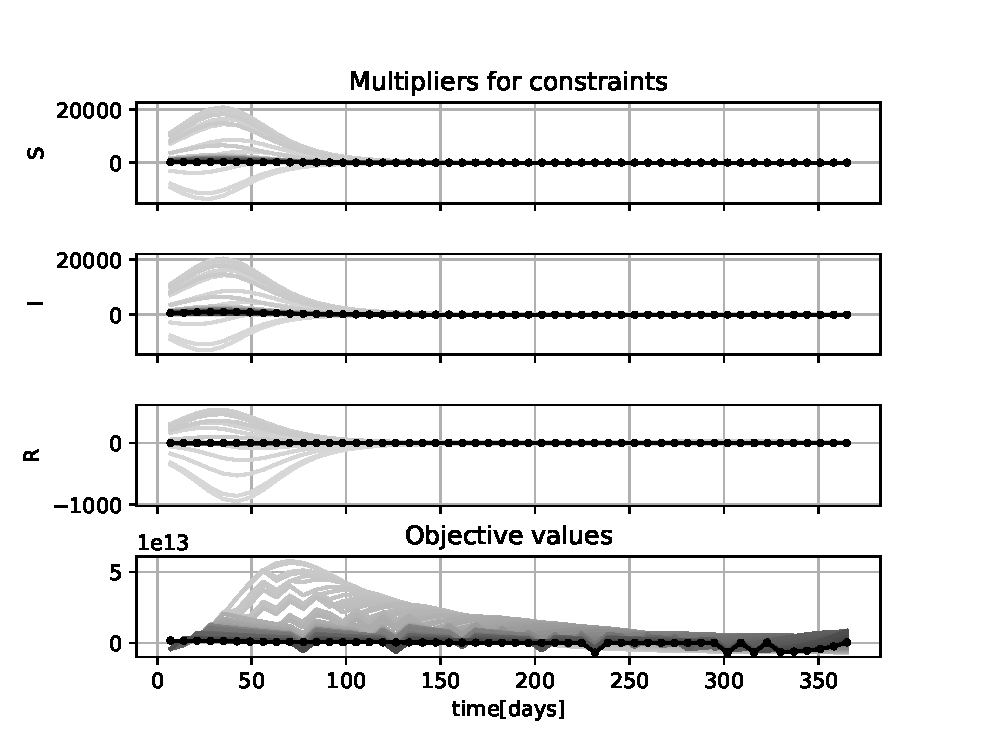
\includegraphics[width=.8\textwidth]{pythonProject/Figures/Multiple_Shooting_obj_con_IPOPT_traj_initial_Social_Distancing.eps}
    \caption{Constraints and objective values multiple shooting using IPOPT (Social Distancing)}
    \label{fig:MS_Cons_Obj_IPOPT}
\end{figure}

Solving the problem with $x_0$ as initial value for all lifted states yields trajectory shown in figure \ref{fig:MS_Traj_IPOPT}.

\begin{figure}[H]
    \centering
    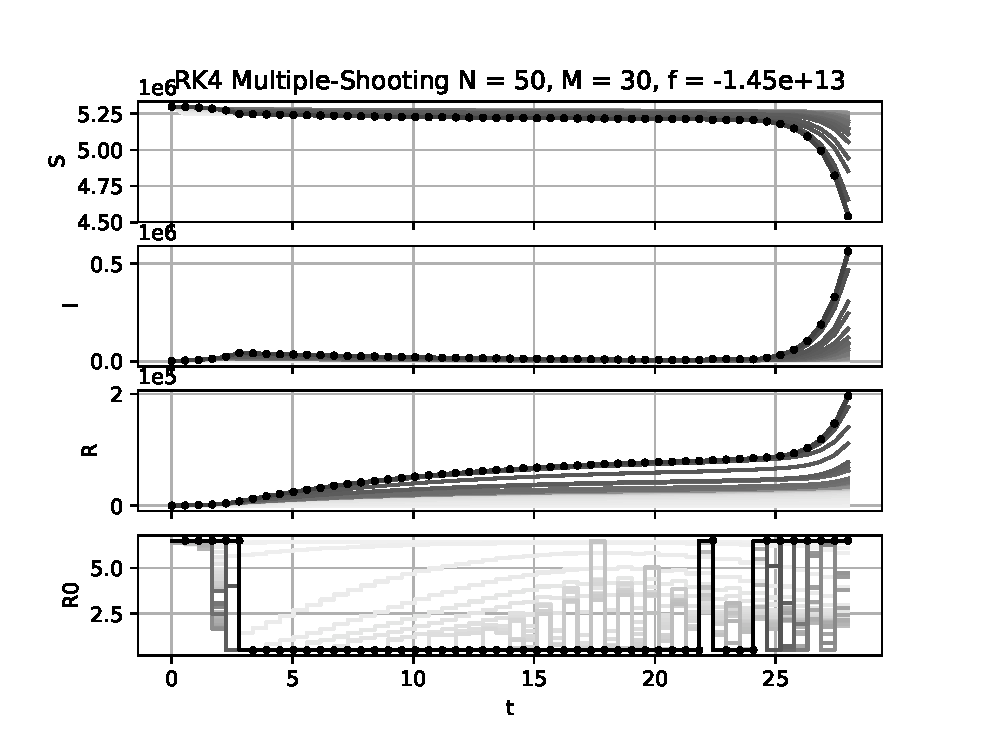
\includegraphics[width=.8\textwidth]{pythonProject/Figures/Multiple_Shooting_Trajectory_IPOPT.eps}
    \caption{Trajectories with multiple shooting using IPOPT (Social Distancing)}
    \label{fig:MS_Traj_IPOPT}
\end{figure}

\subsubsection{Results (Collocation)}


\begin{figure}[H]
    \centering
    \includegraphics[width=.8\textwidth]{pythonProject/Figures/D.eps}
    \caption{Trajectories with multiple shooting using IPOPT (Social Distancing)}
    \label{fig:MS_Traj_SD_IPOPT}
\end{figure}

\subsubsection{Discussion}
The lifted states enables the problem to be solved to a better objective value at the cost of more iterations. The partially concave objective function makes the solver converge towards the same local solution as in single shooting, but postpones the lockdown phase for another day.

Choosing infeasible initial conditions results in a better solution of the problem. By setting all lifted states to $x_0$, the IPOPT-solver converges towards a solution with a much longer lockdown-phase, and is effectively able to avoid an epidemic until the end of the control horizon, where the lockdown policies are lifted. The local solution lifts the lockdown-restrictions for a one-day period before the permanent lifting. This would not have a good effect in reality, but illustrates the need for an objective function rewarding gradual lifting of lockdowns. 



\section{Pontryagin's Maximum Principle}
Optimal control with PMP will consider the continous formulation of the control problem:
\begin{mini*}|s|
{w}{\int_{t=0}^T I(t)^2 -W_u u(t)^2}
{}{}
%\addConstraint{x_f = f(x_0, u(t))}
\addConstraint{\dot{x}(t) = F(x(t), u(t))}
\addConstraint{u_{max} \geq u(t) \geq u_{min}, \quad \forall t \in [0, T)}{}
\end{mini*}
Where $F(.)$ is the SIR ODE-dynamics. The hamiltonian for the problem becomes:
\begin{align}
    H(x, \lambda, u) &= L(I(t), u(t)) + \lambda^T F(x(t), u(t))\\
    = I(t)^2 - W_u &u(t)^2 + (\lambda_1 - \lambda_0)\cdot u(t)\frac{S(t)I(t)}{N_{pop}} + (\lambda_3 -\lambda_1) \alpha I(t)
\end{align}
Minimizing the hamiltonian every timestep will minimize the objective function. In this case it is possible to derive an unconstrained solution:
\begin{align}
    \argmin_u  H(u) &\rightarrow u = \pm \infty %\frac{\partial H(x, \lambda, u)}{\partial u} = 0\\
     %u &= \frac{(\lambda_1-\lambda_0)}{2W_u}\cdot \frac{S(t)I(t)}{N_{pop}}
\end{align}
Constraints $u_{min} \leq u \leq u_{max}$ cannot have the same optimum. However, the concavity of hamiltonian with respect to $u$ ensures that the following holds for constrained $u_c^*(t)$:
\begin{align}
    u^*(t) &= \argmin_u H(x, \lambda, u)\\
    u_c^*(t) &= \begin{cases}
    u_{min} \mbox{ if } u^*(t) < u_{min}\\
    u^*(t) \mbox{ if } u_{min} \leq u^*(t) \leq u_{max}\\
    u_{max} \mbox{ if } u^*(t) > u_{max}
    \end{cases}
\end{align}

\subsection{Single-Shooting Algorithm in CasADI}
The analytical optimal solution for $u$ removes the need for nonlinear optimization and iterations, but CasADI's symbolical framework is still useful for constructing the integrator. 

\begin{algorithm}[H]
\SetAlgoLined
\KwData{$x_k = x_0, u = [u_0, \dots, u_{N-1}], h, N$}
Construct integrator $f(ODE, x, u, h)$ with CasADI-symbolics\\
 \For{$i$ = 0 : $N-1$}{
    $u^*_{c, k} = \argmin_u H(x, \lambda, u)$\\
    $x_k$ = $f(@SIR, x_k, u^*_{c, k}, h)$\\
 }
 \caption{Single-shooting with PMP}
 \label{alg:SingleShooting_Integration_PMP}
\end{algorithm}

\subsection{Simulations}







\end{document}
